\documentclass[11pt]{article}
\usepackage{coling2014}
\usepackage{times}
\usepackage{url}
\usepackage{latexsym}
\usepackage{graphicx}
\usepackage{amsmath}
\usepackage{xcolor}
\usepackage{enumitem}
\usepackage{color}

%\setlength\titlebox{5cm}

% You can expand the titlebox if you need extra space
% to show all the authors. Please do not make the titlebox
% smaller than 5cm (the original size); we will check this
% in the camera-ready version and ask you to change it back.


\title{Modelling of Adjectives in the Ontology-Lexicon Interface}

\author{John P. M\textsuperscript{c}Crae \\
  Affiliation / Address line 1 \\
  Affiliation / Address line 2 \\
  Affiliation / Address line 3 \\
  {\tt email@domain} \\\And
  Francesca Quattri, Christina Unger, Philipp Cimiano \\
  Affiliation / Address line 1 \\
  Affiliation / Address line 2 \\
  Affiliation / Address line 3 \\
  {\tt email@domain} \\}

\date{}

\begin{document}
\maketitle
\begin{abstract}
    The ontology-lexicon interface has become an important and successful tool 
for handling problems in natural language processing. The foundation of these models 
is based on the separation of the ontological and lexical layers by means of the 
principle of semantics by reference to an ontology in description logics. 
However, as noted by other authors, the use of first order logic (hence also description logics),
while effective for nouns and verbs, breaks down in the case of adjectives. 
We propose that this is primarily due to a lack of logical expressivity in the 
ontology. In particular, beyond the straightforward intersective adjectives
many adjectives are i) gradable requiring fuzzy or 
non-monotonic semantics or ii) operator adjectives require second-order logic. 
We consider how we can handle the ontology-lexicon interface in the face of 
these more complex logical formalism, and show how these can be backward 
engineered into OWL based modelling by means of pseudo-classes, with application
to question answering.
\end{abstract}



\section{Introduction}
\label{intro}
\blfootnote{  
     This work is licensed under a Creative Commons 
     Attribution 4.0 International Licence.
     Page numbers and proceedings footer are added by
     the organisers.
     Licence details:
     \url{http://creativecommons.org/licenses/by/4.0/}
}

Ontology-lexicon models, such as \emph{lemon} (Lexicon Model for Ontologies)~
\cite{mccrae2012interchanging}, have become an important model for handling a 
number of tasks in natural language processing. In particular, such 
ontology-lexica are built around the separation of a lexical layer describing 
how a word or phrase acts syntactically and morphologically, and a semantic layer 
describing how the meaning of a word is expressed in a formal logical model, 
such as OWL (Web Ontology Language)~\cite{mcguinness2004owl}. It has been 
shown that this principle known as \emph{semantics by reference}~
\cite{buitelaar2010ontology} is an effective model that can be used in tasks 
such as question answering \cite{unger2011pythia} and natural language 
generation \cite{cimiano2013exploiting}. In particular, its suitability to the 
task is driven by the fact that the application of this model to answering questions 
based on the DBpedia \cite{auer2007dbpedia} knowledge base requires mostly 
understanding the nouns and the verbs of the sentence. However, as has been 
shown by the Question Answering over Linked Data \cite[QALD]{lopez2013evaluating}
tasks, there are many questions that can be asked over this database that require 
a deeper semantic understanding of the representation of language. For example, 
questions such as~\ref{ex:australia} require understanding of the semantics of `high' in a manner that goes beyond 
the model of OWL based on classes, properties and individuals. The answer given 
in the QALD dataset for this question is shown in~\ref{ex:australia_query}. 
In particular, the interpretation of this question involves the understanding of 
how the word `high' relates to the property {\tt dbo:elevation}, including ordering 
and subset selection operations, and how to express this semantics in a formal manner.

\begin{enumerate}
\item \begin{enumerate} 
\item What is the highest mountain in Australia? \label{ex:australia}
\item \begin{verbatim}
SELECT DISTINCT ?uri WHERE { 
  ?uri rdf:type dbo:Mountain . 
  ?uri dbo:locatedInArea res:Australia . 
  ?uri dbo:elevation ?elevation . 
} ORDER BY DESC(?elevation) LIMIT 1
\end{verbatim} 
\label{ex:australia_query}
\end{enumerate}
\end{enumerate}

It has been claimed that first-order logic and thus by extension description 
logics, such as OWL, ``fail decidedly when it comes to adjectives''
\cite{bankston2003modeling} and similarly we reach the conclusion that 
this is due to the issues of semantically modelling adjectives. In fact, we largely agree that the semantics 
of many adjectives are difficult or impossible to describe in first-order logic. 
However, from the point of view of the ontology-lexicon interface, the logical 
expressivity of the ontology is not a limiting factor. In fact, due to the 
separation of the lexical and ontology layers in a model such as \emph{lemon}, 
it is possible to express the meaning of words without worrying about the 
formalism used in the ontology. To this extent, we will first demonstrate that 
adjectives are in general a case where the use of description logics (DL) breaks down, 
and for which more sophisticated logical formalisms must be applied. We then 
consider to what extent this can be handled in the context of the 
ontology-lexicon, and introduce pseudo-classes, that is OWL classes with 
annotations, which we use to express the semantics of adjectives in a manner
that would allow reasoning with fuzzy, high-order models. To this extent, we base
our models on the previously introduced design patterns~\cite{mccrae2014design}
for modeling ontology-lexica. 
Finally, we show how these semantics can be helpful in practical applications 
of question answering over the DBpedia knowledge base.

\section{Classification of adjectives}

There are a number of classifications of adjectives \cite{}. First we will start 
with the most fundamental distinction of \emph{attributive} versus 
\emph{predicative} usage, that is the use of adjectives in noun phrases 
(``$X$ is a $A~N$'') versus as objects of the copula (``$X$ is $A$''). 
It should be noted that there are many adjectives for which only predicative or 
attributive usage is allowed, as shown in~\ref{ex:clinton} and~\ref{ex:baby}.

\begin{enumerate}[resume]
\item \begin{enumerate}	
\item \ \,Clinton is a former president.
\item $^*$Clinton is former.
\end{enumerate}
\label{ex:clinton}
\item \begin{enumerate}	
\item \ \,The baby is awake.
\item $^*$The awake baby.
\end{enumerate}
\label{ex:baby}
\end{enumerate}

One of the principle classifications of the semantics of adjectives (for example \cite{partee2003there,bouillon1999description,morzycki2013modification}) is based on the meaning of adjective noun compounds relative to the meaning of the words by themselves. This classification is as follows (where $\Rightarrow$ denotes entailment).

\begin{description}
\item[Intersective] ($X\mathrm{~is~a~}A~N \Rightarrow X\mathrm{~is~}A \cap  X\mathrm{~is~a~}N$) 
Such adjectives work as if they were another noun and indicate that the compound 
noun phrase is a member of both the class of the noun and the class of the 
adjective. For example, in the phrase ``Belgian violinist'' it refers to a 
person in the class intersection $Belgian \sqcap Violinist(X)$, and hence we 
can infer that a ``Belgian violinist'' is a subclass of a ``Belgian''. 
Thus if we also knew that the ``violinist'' was a ``surgeon'' we could 
conclude they were a ``Belgian surgeon''.
\item[Subsective] ($X\mathrm{~is~a~}A~N \Rightarrow X\mathrm{~is~a~}N$, but $X\mathrm{~is~a~}A~N \not\Rightarrow X\mathrm{~is~}A$) 
Such adjectives do not alter the meaning of the noun phrase itself, but only 
make sense with knowledge of the noun they refer to. For example, a ``skilful 
violinist'' is certainly in the class $Violinist(X)$, but if we knew that that 
person is a surgeon as well, we cannot conclude that the person is a skilful surgeon. 
\item[Privative] ($X\mathrm{~is~a~}A~N \not\Rightarrow X\mathrm{~is~a~}N$) 
These adjectives modify the meaning of a noun phrase to create a noun phrase 
that is potentially incompatible with the original meaning. For example, a 
``fake gun'' is not a member of the class of guns.
\end{description}

This classification is useful, however one further case is important to 
distinguish and that is of \emph{relational} adjectives which have a meaning 
that expresses a relationship between two individuals or events, for example:

\begin{quote}

He is related to her.
\end{quote}

Another important distinction to make with adjectives is whether they are 
\emph{gradable}, in that whether it makes semantic senses to make a comparative 
or superlative statement with these adjectives. For example, adjectives such as 
`big' or `tall' can express relationships such as `$X$ is bigger than $Y$', 
however it is not possible to say one individual is `more former'. Most gradable 
adjectives are subsective, for example `a big mouse' is not `a big animal'\cite{morzycki2013nonscales}. An 
important group of gradable adjectives are, however, intersective, and we call 
such adjectives `absolute' (following \cite{rusiecki1985adjectives}) as they 
refer to an ideal point on some scale, for example a `straight line' is `straight', in 
that it has no bends or kinks, however we can still talk about a line being 
`straighter', in the sense of closer to the ideal of straightness than some other object

Finally, we consider \emph{operator} or \emph{property-modifying} adjectives, 
which can be considered to be the same as privative adjectives, but in this 
case are understood as operators that change some property in the qualia 
structure of the class. For example, we may express the adjective `former' 
in lambda calculus as a function that takes a class $C$ as input and returns the class 
of entities that were a member of $C$ to some prior time point $t$~\cite{partee2003there}:

$$\lambda C [\lambda x \exists t C(x,t) \cap t < \mathrm{now}]$$

Such adjectives have not only a difference in semantic meaning but can also 
frequently have syntactic impact, for example in adjective ordering 
restrictions, as they may be reordered with only semantic 
impact~\cite{teodorescu2006adjective}, e.g.,

\begin{enumerate}[resume]
\item \begin{enumerate}
\item \ A big red car.
\item $^?$A red big car.
\end{enumerate} 
\label{ex:car}
\item \begin{enumerate}
\item A famous former actor.
\item A former famous actor.
\end{enumerate}
\label{ex:actor}
\end{enumerate}

One further case that is important to distinguish is that of \textbf{relational} adjectives which have a meaning 
that expresses a relationship between two individuals or events, for example:

\begin{enumerate}[resume]
\item He is related to her.
\item She is similar to her brother. 
\item This is useful for something. 
\end{enumerate}

Another important distinction to make with adjectives, which is orthogonal to the above classification, 
is whether they are \emph{gradable}, in that whether it makes semantic senses to make a comparative 
or superlative statement with these adjectives. For example, adjectives such as 
`big' or `tall' can express relationships such as `$X$ is bigger than $Y$', 
however it is not possible to say one individual is `more former'. It should thus be noted that most gradable adjectives are mostly intersective,
for example a `big mouse' is not a `big animal' \cite{morzycki2013modification}.
An important group of gradable adjectives are, however, intersective, and we call 
such adjectives \emph{absolute} (following \cite{rusiecki1985adjectives}) as they 
refer to an ideal point on some scale, such as `straight', and frequently refer
to an endpoint of a scale, which Kennedy~\shortcite{kennedy1999scalar} calls
a \emph{trivial standard}.

\section{Representation of adjectives in the ontology-lexicon interface}

In general it is assumed that adjectives form frames with exactly one argument 
except for extra arguments given by adjuncts, typically prepositional phrases. 
Most adjectives are thus associated with a predicative frame, which much
like the standard noun predicate frame\footnote{$X\text{ is a }N$} is stereotyped in English as:

$$X\mathrm{~is~}A$$

For attributive, usage we associate this with a frame, which is stereotyped as,
where the $N?$ argument is not semantically bound, but instead obtained by
syntactic unification with a noun predicate frame.

$$X\text{ is }A~N?$$

As such, when we encounter the attributive usage of an adjective such as in~\ref{ex:juan}, 
we understand this as the realization of two frames, given in~\ref{ex:juan_frames}.

\begin{enumerate}[resume]
\item Juan is a Spanish researcher. \label{ex:juan}
\item \begin{enumerate}
\item Juan is a researcher.
\item Juan is a Spanish $?$.
\end{enumerate}
\label{ex:juan_frames}
\end{enumerate}

Note we do not provide modeling for adjectives that are part of a noun phrase,
such as `polar bear', which we would capture as a normal noun phrase with 
meaning \emph{ursus maritimus}.

\subsection{Intersective adjectives}

Intersective adjectives are the most straightforward class as in many cases they 
can be explained as either being noun-like (denominal adjectives such as 
`Belgian') or verb-like (deverbal adjectives such as `broken'). Intersective 
adjectives have a single argument as with most adjectives and in this case it is 
natural that they refer to classes, which may be event classes such as described 
in \cite{mccrae2014design}. For practical modeling examples we will use the
\emph{lemon} model as it is the most prominent implementation of the 
ontology-lexicon interface.

The primary mechanism of modelling the syntax-semantics interface in the context 
of \emph{lemon} is by means of assigning a \emph{frame} as a \emph{syntactic 
behaviour} of an entry and giving it \emph{syntactic arguments}, which can then 
be linked to the \emph{lexical sense}, which stands in proxy for a true semantic 
frame in the ontology. For example, the modelling of an adjective such as 
`Belgian' can be achieved as follows (depicted in Figure 
\ref{example-belgian})\footnote{We assume that the namespaces are defined for 
the lexicon as {\tt lexicon}, e.g., \url{http://www.example.org/lexicon}
and for the entry, e.g., {\tt belgian} is \url{http://www.example.org/lexicon/belgian#},
other namespaces are assumed to be as usual.}.

\begin{figure}

\includegraphics[width=\textwidth]{belgian-example}
\caption{Modelling of an intersective adjective `Belgian' in \emph{lemon}\label{example-belgian}}
\end{figure}

\begin{verbatim}
lexicon:belgian a lemon:LexicalEntry ;
  lemon:canonicalForm belgian:Lemma ;
  lemon:synBehavior   belgian:AttrFrame , 
                      belgian:PredFrame ;
  lemon:sense         belgian:Sense .

belgian:Lemma lemon:writtenRep "Belgian"@eng .

belgian:AttrFrame lexinfo:attributiveArg belgian:AttrSynArg .
belgian:PredFrame lexinfo:copulativeArg  belgian:PredSynArg .

belgian:sense lemon:reference [ a owl:Restriction ;
                                owl:onProperty dbpedia:nationality ;
                                owl:hasValue dbpedia:Belgium ] ;
              lemon:isA belgian:AttrSynArg , belgian:PredSynArg .
\end{verbatim}

Note, that here we use the external vocabulary LexInfo \cite{cimiano2011lexinfo} 
to define the meaning of the arguments of the frame as the \emph{attributive 
argument}, corresponding to the frame stereotype ``A $[attr]$ X'' and the 
\emph{copulative argument} for the frame stereotype ``X is an A''. Furthermore,
the class of Belgians is not named in our reference ontology DBpedia, so we 
introduce an anonymous class with the axiomatization, 
$\exists\,\text{nationality}.\text{Belgium}$. It is in fact common that the 
referent of an adjective is not named in an ontology and as such we tend to 
model denomial adjectives as classes of the form $\exists\,\text{\em prop}.\text{\em Value}$, 
where $\text{\em Value}$ is the reference of the noun from which the adjective is
derived. This modelling is so common that it has already been encoded as two
patterns, called {\tt IntersectiveObjectPropertyAdjective} and {\tt
IntersectiveDatatypePropertyAdjective}, see McCrae and Unger \shortcite{mccrae2014design}.
Similarly, most deverbal adjectives refer to an event, and as such
a common modelling is of the form $\exists\,\text{\em theme}^{-1}.\text{\em EventClass}$, 
for example `vandalized' may be $\exists\,\text{\em theme}^{-1}.\text{\em VandalismEvent}$.

\subsection{Gradable adjectives}

Gradable adjectives have a number of properties, which differentiate them
from intersective adjectives:

\begin{itemize}
\item They have a comparative constructions with either `-er' or `more' \cite{kennedy1999scalar}:3), c.f. `*less geological', `*more wooden'.
\item Gradable adjectives have a context-dependent truth-conditional variability, meaning that their positive form is the sum of the relation between the degree of the concept possessed by the object (as measured by the predicate) and the context-dependent standard of comparison based on the same concept \cite{kennedy2007vagueness}. It follows that the properties denoted by adjectives like `expensive' or `small' or `big' vary in intensity according to the context (and time) of use. 
\item They are frequently \emph{fuzzy} (or \emph{vague})~\cite{kennedy2007vagueness}.
%\item \textbf{\textcolor{blue}{\textit{absolute} gradable adjectives, like `straight' or `bent' or `red' (to cite your part on colors below), are not vague}}
\item The arguments of gradable adjectives are mapped into abstract representations of measurements or degrees~\cite{kennedy2007vagueness}.
\item There may be a minimum or maximum of this scale, which can be determined
by, for example, whether they can modified by `completely'.
\end{itemize}

As such we define gradable adjectives relative to a particular 
property\footnote{Note in many cases the property is quite abstract such as in 
`breakable'}, that is it is natural to say that `big' refers to 
`size', however it is clear then that `small' also refers to `size' and as antonyms 
they cannot both refer to the same ontological concept. As such, we introduce 
the concept of \emph{covariance} and \emph{contravariance}, which refers to 
whether the comparative form indicates a higher property value for the subject 
or the object. That is that `big' is covariant with size, as bigger things have 
a higher size value, and `small' is contravariant with size. We also introduce 
a third concept of \emph{absolute gradability}, which states that these objects 
are better described by these adjectives as they approach some ideal value. 
A common example of this is colours, which where we may say that some object is 
redder than another if it is closer to some ideal value of red 
(e.g., RGB {\tt 0xff0000}).

\textbf{\textcolor{blue}{On variant and covariant** MORE TO COME}}
  
\textbf{\textcolor{blue}{You introduce here the concepts of covariance and contravariance with reference to antonymic adjectives and the concept they refer to (e.\,g. `big' / `small' and `size'). MORE TO COME}}

While these concepts well handle the comparative usage of adjectives, the 
predicative and superlative usage of adjectives is complicated by three factors 
that we will outline below. We notice that gradable classes are not 
crisply defined as with the case of many intersective adjectives, that is that 
while we can clearly define all people in the world as `Belgian' or 
`not Belgian', by who holds a passport of Belgium, it is not easy 
split the world's population into `tall' and `not tall'. In fact, while it may 
be easy to say that someone with height 6'6'' (198cm) is `tall', it is not clear 
whether someone of height 6' (182cm) is `tall' although they are above average 
height for a man. As such, the class boundary of a gradable adjective is 
naturally fuzzy. Secondly, we note that these class boundaries are 
non-monotonic, that is that with knowledge of more instances of the relative 
class we must revise our class boundaries. This is especially the case for the
superlative as the discovery of a new tallest person in the world would remove 
the existing tallest person in the world from the class of tallest person in the 
world. This, non-monotonicity also affects the class boundaries of the gradable 
class itself, for example in the 18th century the average height of a male was 
5'5'' (165cm).\footnote{\url{https://en.wikipedia.org/wiki/Human_height}}
and as such a male of 6' would have been considered clearly to be 
tall. As such, we can conclude that each instance added to our ontology must 
revise the class boundaries of a gradable class, hence leading to the fact that 
gradable adjectives are fundamentally non-monotonic. Finally, we must notice 
that gradability can only be understood relative to the class that we wish to 
grade, that is that while it is unclear as to whether 6' is tall for a male, 
given the current average height of a female of about 5'4'' (162cm) it is clear 
that 6' is tall for a female.

So we can conclude that gradable adjectives are \emph{fuzzy}, \emph{non-monotonic} 
and \emph{context-sensitive}, all of which are incompatible with the description 
logic used by OWL. Currently there are only limited models for representing fuzzy 
logic in the context of the web~\cite{zhao2008uncertainty}. In order to capture the 
properties of gradable adjectives, we introduce a new model, which we name 
\emph{lemonOILS} (The \emph{lemon} Ontology for the Interpretation of Lexical Semantics)
\footnote{\url{http://lemon-model.net/oils}}. This ontology introduces three 
new classes:

\begin{itemize}
	\item {\tt CovariantScalar}, indicating that the adjective is covariant with its bound property
	\item {\tt ContravariantScalar}, indicating that the adjective is contravariant with its bound property
	\item {\tt AbsoluteScalar}, indicating that the property represents similarity to an absolute value
\end{itemize}

In addition, the following properties are introduced to enable the description 
of gradable adjectives. Note, that all of these properties are typed as 
\emph{annotation properties} in the OWL ontology, so that they do not interfere 
with the standard OWL reasoning.

\begin{itemize}
	\item {\tt boundTo} indicates the property that a scalar refers to (e.g., `size' for `big')
	\item {\tt threshold} specifies a sensible minimal value for which the adjective can be said to hold
	\item {\tt degree} is one of {\tt weak}, {\tt medium}, {\tt strong} or {\tt very strong}, corresponding to approximately 50\%, 25\%, 5\% or 1\% of all known individuals
	\item {\tt comparator} indicates an object property that is equivalent to the comparison of the adjective (e.g., an object property {\tt biggerThan} may be considered a comparator for the adjective class {\tt big})
	\item {\tt measure} (TODO)
	\item {\tt defaultValue} (TODO)
\end{itemize}

Using such classes we can capture the semantics of gradable adjectives 
syntactically but not formally within an OWL model, as such we call such 
introduced classes \emph{pseudo-classes}. An example of modelling an adjective 
such as `high' is given below (depicted in Figure \ref{high-example}).

\begin{figure}
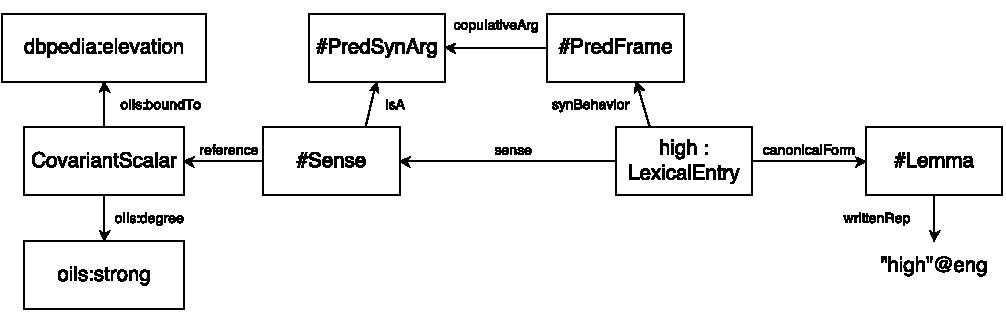
\includegraphics[width=\textwidth]{high-example}
\caption{An example of the modelling of `high' in \emph{lemon}\label{high-example}}
\end{figure}

\begin{verbatim}
lexicon:high a lemon:LexicalEntry ;
  lemon:canonicalForm high:Lemma ;
  lemon:synBehavior high:PredFrame ;
  lemon:sense high:Sense .

high:Lemma lemon:writtenRep "high"@eng .

high:PredFrame lexinfo:copulativeArg high:PredArg .

high:Sense lemon:reference [
    rdfs:subClassOf oils:CovariantScalar ;
    oils:boundTo dbpedia:elevation ;
    oils:degree oils:strong ] ;
  lemon:isA high:PredArg .
\end{verbatim}

As an example of a way in which it would be possible to interpret these 
annotations, we consider Markov Logic~\cite{richardson2006markov}, which is an 
extension of first-order logic in which each clause is given a cost. The process 
of reasoning is thus transformed into an optimization problem of finding the 
extension, which minimizes the summed weight of all violated clauses. As such we
can formulate a gradable adjective based on the number of known instances. 
For example, we can specify `big' w.r.t. \emph{size} for some class $C$ as in~\ref{ex:big}.
%
\begin{enumerate}[resume]
\item $\forall x \in C, y \in C : size(x) > size(y) \rightarrow big_C(x) : \alpha$ \\
$\forall x \in C, y \in C : size(x) < size(y) \rightarrow \neg big_C(x) : \beta$
\label{ex:big}
\end{enumerate}
%
In this way, the classification of an object into big or small can be defined as follows.
For an individual $x \in C$ the property $big_C(x)$ holds if and only if: 

$$|\{y \in C, size(y) > size(x)\}| \alpha < |\{y \in C, size(y) < size(x)\}| \beta$$

Where the values of $\alpha$ and $\beta$ are related to the degree defined
in the ontology.

We see that `big' defined in this way has the three properties outlined above: 
it is non-monotonic (in that more individuals may change whether we consider an individual 
to be `big' or not), it is fuzzy (given by the strength of the probability of the proposition $big_C(x)$), 
and it is context-sensitive (as whether an individual counts a big or not depends on the class $C$).

\textbf{Thresholds, defaults and multiple classes (Francesca to help)}

\subsection{Operator adjectives}

Operator adjectives are those that combine to alter the meaning of the adjective itself. 
There are two primary issues with the understanding of the adjective in this manner. 
Firstly, the reference of the lexical item does not directly refer to an existing item 
in the ontology, but rather is novel and productive. Secondly, the compositional nature 
of adjective-noun compounds is no longer simple as in the cases of intersective and gradable adjectives. 
To this extent we claim that it is not generally possibly to represent the 
meaning of an operator adjective, within the context of an OWL ontology.
Instead, following Bankston~\cite{bankston2003modeling}, we claim that
the reference of an operator adjective must be a higher order predicate.
If we assume that there are operators of the form of a function, then
the argument of a operator is then the attributed noun phrase, as such
we introduce a frame \emph{operator attributive}, that has one argument
which is the noun. As such the interpretation of a phrase such as

\begin{quote}
Clinton is a former president.
\end{quote}

Is understood as:

\[
[former(President)](Clinton)
\]

Where $former$ applies to $President$ to create a new class in the ontology.
As there is at the moment no agreed representation for such an operator in an
ontology, it underlines the fact that more sophisticated ontology representations than first-order logic are required to understood natural
language in general.

\textbf{this kind of wusses out, but what else can we do?}

%This means that we must acknowledge operator adjectives in both the lexicon and the ontology. 
%To this extent we define a frame called operator adjective frame, whose prototype is:
%
%$$X\mathrm{~is~a~}A~NP$$
%
%This leads to the odd case that operator adjectives are then considered the 
%head of the frame! \textbf{hmm...} In this case 
%we can understand the reference of the adjective as a property that relates an 
%individual to a class. As such it is clear, that the reference of an operator 
%adjective is a higher-order predicate. Fortunately, in the case of OWL we can 
%cheat on this second-order nature by means of \emph{punning}, which allows a 
%class to also be an individual. If we thus assume that operator adjectives are 
%essentially puns, then it follows that we can assume that the reference of an 
%operator adjective is thus a property. As such, for example, we can model an 
%adjective such as `former' as referring to a property such as {\tt heldRole} 
%whose range is a class of roles punned as individuals. This approach is 
%effective, however it has limits in general \textbf{does it???}
%
%We will not be able to easily create a vocabulary that can fully describe the 
%semantics of the adjective within the context of OWL as the second nature order 
%of the logic cannot be captured well within the framework of description logic. 
%However, we can use the punning trick described above to capture the semantics
%of the adjective. To do this we need to add a frame on the syntax side, that 
%indicates that the argument of the adjective is in fact the noun phrase. We 
%would do this as follows (see also Figure \ref{former-example}):
%
%\begin{figure}
%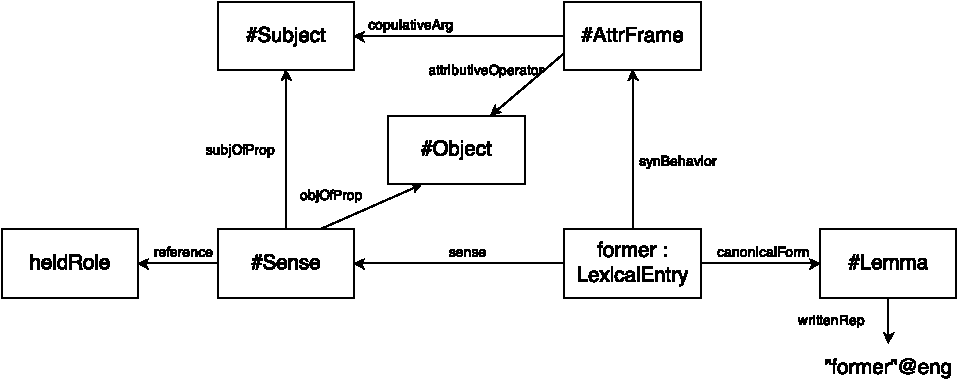
\includegraphics[width=\textwidth]{former-example}
%\caption{An example of modelling `former' in %\emph{lemon}\label{former-example}}
%\end{figure}
%
%\begin{verbatim}
%former: a lemon:LexicalEntry ;
%	lemon:canonicalForm former:Lemma ;
%	lemon:synBehavior former:OperatorFrame ;
%	lemon:sense former:Sense .
%
%former:Lemma lemon:writtenRep "former"@eng .
%
%former:OperatorFrame lexinfo:copulativeArg former:Subject ;
%  lexinfo:attributiveOperator former:Object .
%  
%former:Sense lemon:reference onto:heldRole ;
%  lemon:subjOfProp former:Subject ;
%  lemon:objOfProp former:Object .
%\end{verbatim}
%
%The usage of this frame is intended such that a phrase such as:
%
%\begin{quote}
%Clinton is a former president
%\end{quote}
%
%Is interpreted as:
%
%\begin{verbatim}
%ontology:Clinton ontology:heldRole ontology:President .
%\end{verbatim}

\subsection{Relational adjectives}

Relational adjectives are among the simplest and modelled with another frame,
which extends the attributive frame by allowing for a prepositional phrase
adjunct. As such we can model `known' with the frame `$X$ is known to $Y$' and
reference {\tt foaf:knows} as:

\begin{verbatim}
lexicon:known a lemon:LexicalEntry ;
  lemon:canonicalForm known:Lemma ;
	lemon:sense known:Sense ;
	lemon:synBehavior known:Frame .

known:Lemma lemon:writtenRep "known"@eng .

known:Frame lexinfo:attributeArg known:Subject ;
  lexinfo:prepositionalObject known:Object .

known:Sense lemon:reference foaf:knows ;
  lemon:subjOfProp known:Subject ;
	lemon:objOfProp known:Object .
	
known:Object lemon:marker lexicon:to .
\end{verbatim}


\section{Adjectives in question answering}

Most common adjective kinds in QALD-4:

\textbf{Intersective adjectives}

\begin{itemize}
\item denoting a restriction class, e.g.
 \begin{itemize}
 \item Danish films ($\exists\,\texttt{dbo:country}.\texttt{res:Denmark}$)
 \item female given names ($\exists\,\texttt{dbo:gender}.\texttt{res:Female}$)
 \item Methodist politicians ($\exists\,\texttt{dbo:religion}.\texttt{res:Methodism}$)
 \end{itemize}

\item empty semantic contribution, e.g.
 \begin{itemize}
 \item official website (\texttt{dbo:website})
 \item artistic movement (\texttt{dbo:movement})
 \item national anthem (\texttt{dbo:anthem})
 \end{itemize}

\item non-separable semantic contribution (whole NP corresponds to class or property), e.g.
 \begin{itemize}
 \item American inventions (\texttt{yago:AmericanInventions})
 \item official languages (\texttt{dbo:officialLanguages})
 \item military conflicts (\texttt{dbo:battle})
 \end{itemize}
\end{itemize}


\textbf{Subsective adjectives}

\begin{itemize}
\item denoting a property
 \begin{itemize}
 \item professional (\texttt{dbo:occupation}, as opposed to hobby)\\
       e.g. professional surfer = $\exists\,\texttt{dbo:occupation}.\texttt{res:Surfing}$
 \end{itemize}
\end{itemize}

\textbf{Privative adjectives}

\begin{itemize}
\item not treated 
 \begin{itemize}
 \item former Dutch queen Juliana = \texttt{res:Juliana}
 \end{itemize}
\end{itemize}


\textbf{Gradable adjectives}

\begin{itemize}
\item positive form only occurs with \texttt{how}, denoting a property, e.g.
 \begin{itemize}
 \item how deep (\texttt{dbo:depth})
 \item how heavy (\texttt{dbo:mass})
 \item how tall (\texttt{dbo:height})
 \item how high (\texttt{dbo:elevation})
 \end{itemize}
\item comparative denotes a property plus aggregation, e.g. 
 \begin{itemize}
 \item higher than (\texttt{dbo:elevation} + \texttt{FILTER} with comparision operator that depends on polarity) 
 \item earlier than (\texttt{dbo:date} or \texttt{year} + \texttt{FILTER} with comparision operator that depends on polarity)
 \end{itemize}
\item superlative denotes a property plus aggregation, e.g. 
 \begin{itemize}
 \item the highest (\texttt{dbo:elevation} + \texttt{ORDER BY DESC($\cdot$) OFFSET 0 LIMIT 1}) \\
       the second highest (\texttt{dbo:elevation} + \texttt{ORDER BY DESC($\cdot$) OFFSET 1 LIMIT 2})
       the highest after (\texttt{dbo:elevation} + \texttt{FILTER} + \texttt{ORDER BY DESC($\cdot$) OFFSET 0 LIMIT 1})
 \item the longest (\texttt{dbo:length} + \texttt{ORDER BY DESC($\cdot$) OFFSET 0 LIMIT 1}) 
 \item the youngest (\texttt{dbo:birthDate} + \texttt{ORDER BY DESC($\cdot$) OFFSET 0 LIMIT 1})
 \item the most frequent (ordering \texttt{COUNT})
 \end{itemize}
\item superlative denotes an aggregation operation (whereas the property is contributed by the noun)
 \begin{itemize}
 \item highest population density 
 \item lowest rank 
 \item longest span 
 \end{itemize}
\item superlative has a non-separable contribution 
 \begin{itemize}
 \item the highest place (\texttt{dbo:highestPlace}) 
 \end{itemize}
\end{itemize}


\textbf{Others}

\begin{itemize}
\item temporal
 \begin{itemize}
 \item first album (\texttt{releaseDate} + \texttt{ORDER BY ASC($\cdot$) OFFSET 0 LIMIT 1})
 \item first president ($\exists\,\texttt{dbo:office}.\text{`1st President of the United States'}$)
 \item past two years (\texttt{year} + \texttt{FILTER})
 \end{itemize}
\item first season ($\exists\,\texttt{dbo:seasonNumber}.1$)
\item alive (\texttt{deathDate} + \texttt{FILTER !BOUND})
\end{itemize}



\section{Related work}

The categorization of adjectives in terms of formal semantics goes back to Montague\shortcite{montague1970english} and Vendler\shortcite{vendler1968adjectives}, however one of the most significant attempts to assign a formal meaning was carried out in the Mikrokosmos project\cite{raskin1995lexical}. This was one of the first works to treat the case of a micro-theory of adjectives, in which the results were ``machine-tractable'', in that they could be formally defined by a computer. The applications of this were limited however and no formal logic was attached to the semantic representations, nevertheless much of the modelling resembles ours. In particular, scalar adjectives are modelled by association with an attribute and a range, e.g., `big' was described as being {\tt >0.75} (i.e., 75\% of all known instances) on the {\tt size-attribute}. These classifications do not however clearly separate meaning and syntax and as they also required a seperate modelling of comparatives and class-specific meanings for many adjectives.

Amoia and Garden~\shortcite{amoia2006adjective} handled the problem of adjectives in the context of textual entailment and they analyzed 15 classes that show the subtle interaction between the semantic class (e.g., `privative') and the issues of attributive/predicative use and gradability. 

Abdullah and Frost~\shortcite{abdullah2005adjectives} tackles the privative nature of adjectives by arguing that the adjectives modify the set themselves, in a manner that is naturally second-order. Similarly, Partee~\shortcite{partee2003there} proposed a limited second-order model by means of their `head primary principle' requiring that adjectives are interpreted within their context. The analysis of Bankston~\shortcite{bankston2003modeling} however shows that the fundamental nature of many adjectives is higher-order, and provides a very sophisticated formal representation framework for this syntactic class.

The Generative Lexicon~\cite{pustejovsky1991generative} provides another approach to the representation of semantics, and the case of adjectives has also been considered in this context. Bouillion~\shortcite{bouillon1999adjective} consider the case of the French adjective `vieux' (`old'), which he interprets as selecting two different
elements in the event structure of an attributed noun, that is whether the
state, e.g., being a `mayor' for `mayor', is considered old or the individual
itself. In this way, the introduction of two senses for `vieux' is avoided, 
however it remains unclear if such reasoning introduces more complexity than
the the extra senses.

\cite{morzycki2013modification}

\cite{mcnally2004relational}

Peters and Peters~\shortcite{peters2000treatment} provide one of the few other practical reports on modelling adjectives with ontologies, in the context of the SIMPLE lexica. This work is primarily focussed on the categorization of by means of intensional and extensional properties, rather than due to their logical modelling. 

\section{Conclusion}

In this paper we have presented a method for modelling adjectives with the
ontology-lexicon model, \emph{lemon}. In particular, we found that adjectives
frequently go beyond the first-order logic model used by OWL, but instead 
require models that are non-monotonic, fuzzy and second-order. As such, we 
conclude that more sophisticated semantic models are required to represent the semantics
of such words, however the separation of syntax and semantics remains a robust
model, which can easily be adapted to the task of representing adjectives. As 
a final note we consider the fact that not all languages even have adjectives
\cite{?} and as such we must wonder to what extent this analysis is applicable
beyond English. We contend, that the underlying semantics of the words we discuss here
is representable in all nearly languages and based on our analysis of realistic
questions as applied in QALD, we believe that this model should be applicable
to a range of domains and languages with little issue, however further 
validation is naturally necessary.

\section*{Acknowledgements}

\bibliographystyle{acl}
\bibliography{cogalex-adjectives}

\end{document}
